% \documentclass[serif]{beamer} % Serif for Computer Modern math font.
\documentclass{beamer} % Handout mode to ignore pause statements
\hypersetup{colorlinks,linkcolor=,urlcolor=red}
\setbeamertemplate{navigation symbols}{} % Supress navigation symbols
\usetheme{Berlin} % Displays sections on top
\usepackage[english]{babel}
\usepackage[normalem]{ulem}
\usepackage[makeroom,thicklines]{cancel}
\usepackage{natbib}
\usepackage{subfigure}
\usepackage{hyperref}
\hypersetup{colorlinks,linkcolor={blue},citecolor={blue},urlcolor={red}}  
\newcommand{\mb}[1]{\boldsymbol{#1}}
\newcommand{\bracevec}[1]{\left\lbrace #1 \right\rbrace}
\setlength{\arraycolsep}{2pt} % default: 5pt
\medmuskip = 1mu % default: 4mu plus 2mu minus 4mu
% \definecolor{links}{HTML}{2A1B81}
% \definecolor{links}{red}

\setbeamertemplate{footline}[frame number] 

\mode<presentation>
% \mode<handout>{\setbeamercolor{background canvas}{bg=black!5}}







\def\[#1\]{\begin{equation}\begin{aligned}#1\end{aligned}\end{equation}}
\def\*[#1\]{\begin{align*}#1\end{align*}}

\title{\textbf{Bayesian smoothing with extended second order random walk model: An detailed overview and comparison}}

\author{Ziang Zhang\\[5mm]{\small Supervisors: Patrick Brown \\ \hspace{18mm} James Stafford}}



\institute{Department of Statistics, University of Toronto}
\date{2020-05-06}

\date{November 2021}


\setbeamercovered{transparent}

\begin{document}

\begin{frame}
\titlepage
\end{frame}

\begin{frame}
\frametitle{Outline}
\tableofcontents
\end{frame}

\section{Introduction}
\subsection{Why Bayesian smoothing spline?}
\begin{frame}
\begin{block}{Smoothing Spline Problem}
Consider a data set $\{y_i,x_i, i\in [n]\}$, and a nonparametric model $y_i = g(x_i) + \epsilon_i$ where $\epsilon_i \overset{iid}\sim N(0,\sigma_\epsilon^2)$ and $x_i \in [a,b]$, then the (traditional) smoothing spline aims to solve the following problem:
\pause
\begin{equation}\label{equ:ss}
\arg\min_{g\in C^2} \bigg\{ \sum_i \bigg(\frac{y_i-g(x_i)}{\sigma_\epsilon}\bigg)^2 + \lambda  \int_a^b g''(x)^2 dx \bigg\}
\end{equation}
\pause
The sum of square term on the left can be replaced by negative log likelihood, which is also called \textit{penalized likelihood} method.
\end{block}

\pause

\textbf{Question:} How to incorporate the uncertainty from estimating $\sigma_\xi$ and $\lambda$ into  the inferences?

\pause

\textbf{One Solution:} Bayesian hierarchical model, which provides model-based estimation and uncertainty quantification for all the parameters.

\end{frame}

\begin{frame}

\begin{block}{Vectorized expression of smoothing spline:}
Using the property of natural cubic spline, the term $\int_a^b g''(x)^2 dx$ for any natural cubic spline $g(.)$ can be written as $\boldsymbol{g}^T K \boldsymbol{g}$.
Therefore, the equation \ref{equ:ss} can be written in the following vector form:
\pause
\begin{equation}\label{equ:vectorss}
\frac{1}{ \sigma_\epsilon^2}(\boldsymbol{y} - \boldsymbol{g})^T (\boldsymbol{y} - \boldsymbol{g}) + \lambda \boldsymbol{g}^T K \boldsymbol{g}.
\end{equation}
\end{block}

\pause

Consider without the loss of generality that covariates are equally spaced, then the matrix $K$ can be factorized as the following:
\pause
\begin{equation}\label{equ:ArimaPrior}
K = D^T R^{-1} D.
\end{equation}

\pause

The $(n-2) \times n$ matrix $D$ is a second-order differencing matrix, and the $(n-2) \times (n-2)$ matrix $R^{-1}$ can be shown to correspond to the precision matrix of a MA(1) process \citep{ARIMA}.



\end{frame}


\subsection{Exact method with ARIMA prior}
\begin{frame}
Specifically when covariates are unit spaced, we have the following expressions for $D$ and $R$:
\pause
\begin{equation}
\begin{aligned}
D = \mbox{\scriptsize $\begin{bmatrix}
1 & -2 & 1 & 0 & 0 & \cdots & 0\\
0 & 1 & -2 & 1 & \cdots & 0 & 0\\
0 & \vdots &  &  & \ddots & 0 & 0\\
0 & 0 & 0 & \cdots & 1 & -2 & 1\\
\end{bmatrix}$}, \ 
R = \mbox{\scriptsize $\begin{bmatrix}
\frac{2}{3} & \frac{1}{6} & 0 & 0 & 0 & \cdots & 0\\
\frac{1}{6} & \frac{2}{3} & \frac{1}{6} & 0 & 0 & \cdots & 0\\
0 & \frac{1}{6} & \frac{2}{3} & \frac{1}{6} & 0 & \cdots & 0\\
 &  &  &  &  & \ddots & \\
0 & 0 & 0 & \cdots & 0 & \frac{1}{6} & \frac{2}{3}\\
\end{bmatrix}$}
\end{aligned}
\end{equation}

\pause

\textbf{Problem:} This ARIMA(0,2,1) prior interpretation of smoothing spline will only be valid when all locations are equally spaced. Otherwise the locations should be refined into finer equally spaced resolution first.

\pause

\textbf{Problem:} $R^{-1}$ will be a dense matrix, and hence the precision matrix of $\boldsymbol{g}$ will be a dense matrix as well. Computation will be hard and not compatible with inference method such as Integrated Nested Laplace Approximation(INLA) \citep{inla}.



\end{frame}

\section{Extended RW2 method}

\subsection{SDE-based prior}
\begin{frame}

\begin{enumerate}

\item From result of \cite{wahba}, there is a well known connection between smoothing spline and folded Wiener process prior:
\pause

\item Let $W(t)$ denote the standard Wiener's process (Brownian motion), a SDE based prior is assigned to $g(t)$ in the following way ($\sigma_s = 1/\sqrt{\lambda}$):
$$\frac{d^2g(t)}{dt^2} = \sigma_s\frac{dW(t)}{dt}.$$ 
\pause


\item The derivative of $W(t)$ does not exist in ordinary definition, but can be defined as a generalized function, the \textit{white noise} process. 

\pause


\item If $g(0)$ and $g'(0)$ are given diffuse Gaussian prior, the limiting posterior mean of $\boldsymbol g$ will be the minimizer of the smoothing spline problem \citep{wahba}.

\end{enumerate}

\end{frame}
\subsection{Finite element method}
\begin{frame}

\begin{definition}[Finite Element Method]
Let $\mathbb{B}_p:=\{\varphi_i, i \in [p] \}$ denote the set of $p$ pre-specified basis functions, and let $\mathbb{T}_q:=\{\phi_i, i \in [q]\}$ denote the set of $q$ pre-specified test functions. The finite element approximation $\tilde{g}(.)$ to the true function $g(.)$ is defined as:
\pause
\begin{equation}\label{discretization}
\tilde{g}(.) = \sum_{i=1}^{p}w_i \varphi_i(.),
\end{equation}
\pause
where $\boldsymbol{w} := (w_1,...,w_p)^T \in \mathbb{R}^p$ is a set of weights that satisfies:
\pause
\begin{equation}\label{weakSol}
\langle \frac{d^2\tilde{g}(t)}{dt^2} , \phi_i(t)\rangle \overset{d}= \langle \sigma_s\frac{dW(t)}{dt} , \phi_i(t)\rangle,
\end{equation}
for any test function $\phi_i \in \mathbb{T}_q$.
\end{definition}

\end{frame}
\subsection{Extended RW2}
\begin{frame}

\begin{itemize}

\item \cite{rw2} applied the finite element method above to approximate the SDE-based prior, setting both $\mathbb{B}_p$ and $\mathbb{T}_q$ to be the set of $n$ first order B-spline basis with knots at the covariate values.

\pause

\item This results in the weights parameter $\boldsymbol{w}$ being jointly normal with precision matrix $H^TB^{-1}H$. The matrices $H$ and $B$ are $n \times n$ defined with $H_{ij} = [\langle \frac{d^2\phi_j(t)}{dt^2} , \phi_i(t)\rangle]$ and $B_{ij}=[\langle \phi_i ,\phi_j\rangle]$.

\pause

\item The matrices $H$ and $B$ equal to the matrices $D$ and $R$ in the ARIMA representation, except at the boundaries. They will be exactly equal if we remove $\phi_1$ and $\phi_n$ from the set of test functions an reapply the finite element method.

\pause

\item \cite{rw2} then approximate the tri-diagonal matrix $B$ with its diagonal approximation $A$, which distributes the off-diagonal values in B back to its main diagonal.

\end{itemize}

\end{frame}


\begin{frame}
\begin{itemize}
\item The resulting \textit{approximated} finite element representation is called the extended RW2 model, which generalizes the traditional RW2 model defined for regularly spaced locations \citep{rue2005gaussian}.

\pause

\item Also, because of the diagonal approximation it utilized, the precision matrix will be sparse and hence compatible with inference method such as INLA.
\end{itemize}
\end{frame}


\section{Computations}
\begin{frame}
We implemented and compared the two Bayesian smoothing methods using the following procedures:

\begin{itemize}
\pause
\item Re-parametrizing the smoothing parameter $\sigma_s^2$ as $\theta = -2\log \sigma_s$, and for each value of $\theta$ let $Q_\theta$ denotes the precision matrix corresponding to the evaluation vector $\boldsymbol{g}$.
\pause
\item The conditional posterior $\pi(\boldsymbol{g}|\boldsymbol{y},\theta)$ then is approximated by its Gaussian approximation:
\begin{equation}\label{GaussianApproxi}
\tilde{\pi}_G(\boldsymbol{g}|\boldsymbol{y},\theta) \propto \exp \bigg\{ -\frac{1}{2} \bigg(\boldsymbol{g} - \hat{\boldsymbol{g}}_\theta \bigg)^T H_\theta (\hat{\boldsymbol{g}}_\theta) \bigg(\boldsymbol{g} - \hat{\boldsymbol{g}}_\theta \bigg) \bigg\},
\end{equation}
the quantity $\hat{\boldsymbol{g}}_\theta$ denotes $\text{argmax}_g \log \pi (\boldsymbol{g} | \theta, \boldsymbol{y})$ and $H_\theta (\boldsymbol{g})$ denotes $-\frac{d^2}{d\boldsymbol{g}d\boldsymbol{g}^T} \log \pi(\boldsymbol{g} | \theta, \boldsymbol{y})$.
\end{itemize}
\end{frame}

\begin{frame}


\begin{itemize}
\pause
\item Then, we will follow the procedures as in \cite{tierney1986accurate}, to obtain the Laplace approximation of the posterior of the smoothing parameter $\theta$:
\begin{equation}\label{LaplaceApproxi}
\tilde{\pi}_\text{LA}(\theta|\boldsymbol{y}) \propto \pi(\theta) \bigg\{\frac{|Q_\theta|}{|H_\theta(\hat{\boldsymbol{g}}_\theta)|} \bigg\}^{1/2} \exp \bigg\{ -\frac{1}{2}  \hat{\boldsymbol{g}}_\theta^T Q_\theta  \hat{\boldsymbol{g}}_\theta + l(\boldsymbol{y};\hat{\boldsymbol{g}}_\theta) \bigg\}.
\end{equation}

\pause
\item For the posterior of $\boldsymbol{g}$, we will use the following approximation:
\begin{equation}\label{finalApproxi}
\tilde{\pi}(\boldsymbol{g}|\boldsymbol{y}) = \sum_{k=1}^K \tilde{\pi}_G(\boldsymbol{g}|\boldsymbol{y}, \theta_k) \tilde{\pi}_{\text{LA}}(\theta_k|\boldsymbol{y}) \delta_k,
\end{equation}
where $\{\theta_k, \delta_k\}_{k=1}^K$ is a set of $K$ nodes and weights selected using Adaptive Gauss-Hermite Quadrature (AGHQ) rule \citep{aghq}. 
\pause
\item The computation of the AGHQ rule requires optimization of $\tilde{\pi}_\text{LA}(\theta|\boldsymbol{y})$, which will be done through the TMB package \citep{kristensen2015tmb} with automatic differentiation.


\end{itemize}

\end{frame}

\section{Examples}

\subsection{Simulation Studies}
\begin{frame}

\begin{itemize}
\item Assume the following true data generating process:
$$y_i = g(x_i) + \epsilon_i, $$
where $\epsilon_i \sim N(0,3)$ and $g(x) = 5\sin(0.1x),$ observed at $x \in [0,100]$.


\pause
\item There are 10 equally spaced unique covariate values each with 10 repeated measurements. 

\pause
\item For both methods, we utilized the same penalized complexity prior \citep{simpson2017penalising} for $\sigma_s^2$ and $\sigma_\epsilon^2$, such that $P(\sigma_s > 2) = P(\sigma_\epsilon > 2) = 0.5$. 

\pause
\item We infer the values of $g$ at a high resolution grid $\{z_i\}_{i=1}^{200}$ of equally spaced set of locations in $[0,100]$ with spacing 0.5. We assume the function $g(.)$ can be well approximated by the step function $\tilde{g}(.) = \sum_{i=1}^{200} \mathbb{I}(z_{i}\leq.< z_{i+1})g(z_i)$ where $z_{201} := +\infty$.

\end{itemize}


\end{frame}

\begin{frame}

\begin{figure}[p]
    \centering
    \subfigure[$g$ inferred using RW2]{
      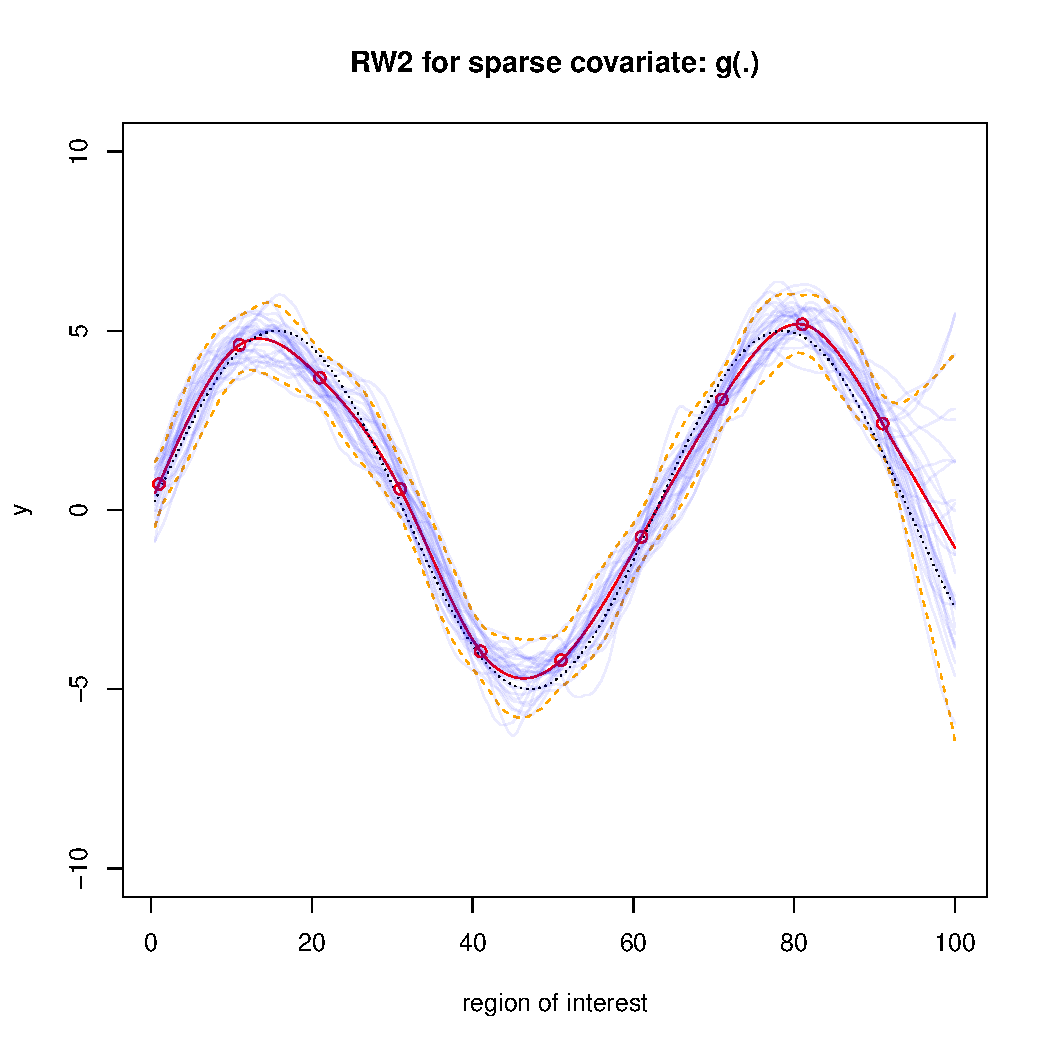
\includegraphics[width=0.27\textwidth]{sim1-g-RW2.pdf}
    }
    \subfigure[$g'$ inferred using RW2]{
      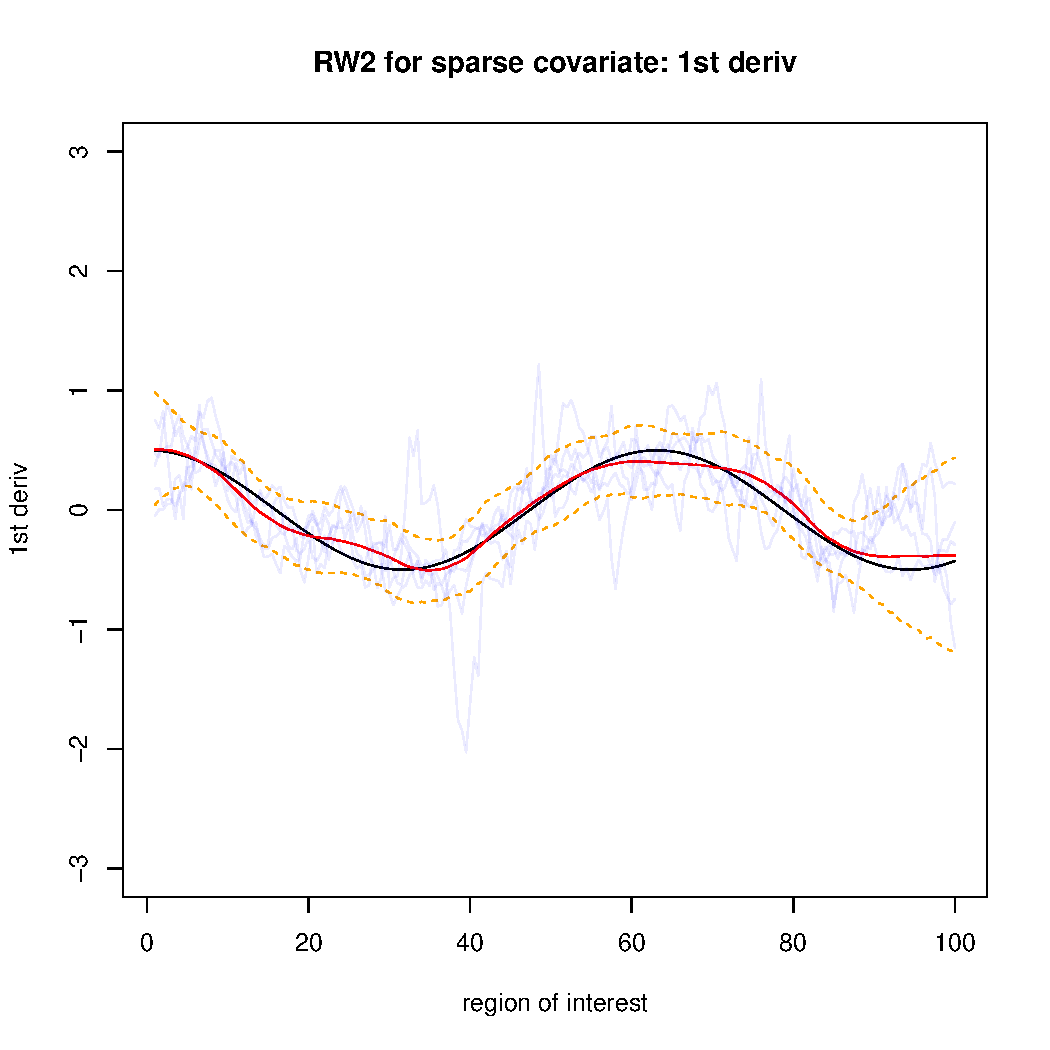
\includegraphics[width=0.27\textwidth]{sim1-g1st-RW2.pdf}
    }
        \subfigure[$g''$ inferred using RW2]{
      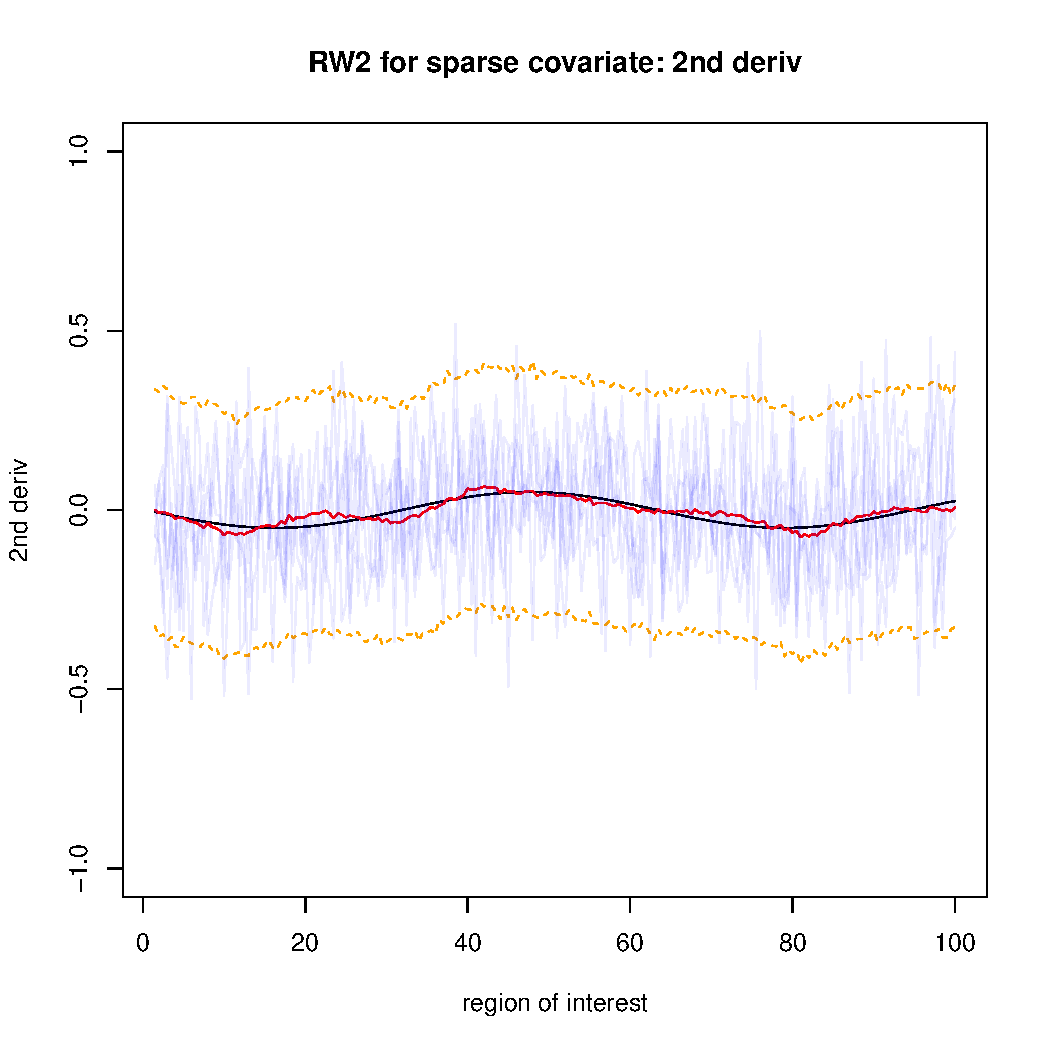
\includegraphics[width=0.27\textwidth]{sim1-g2nd-RW2.pdf}
    }
            \subfigure[$g$ inferred using ARIMA]{
      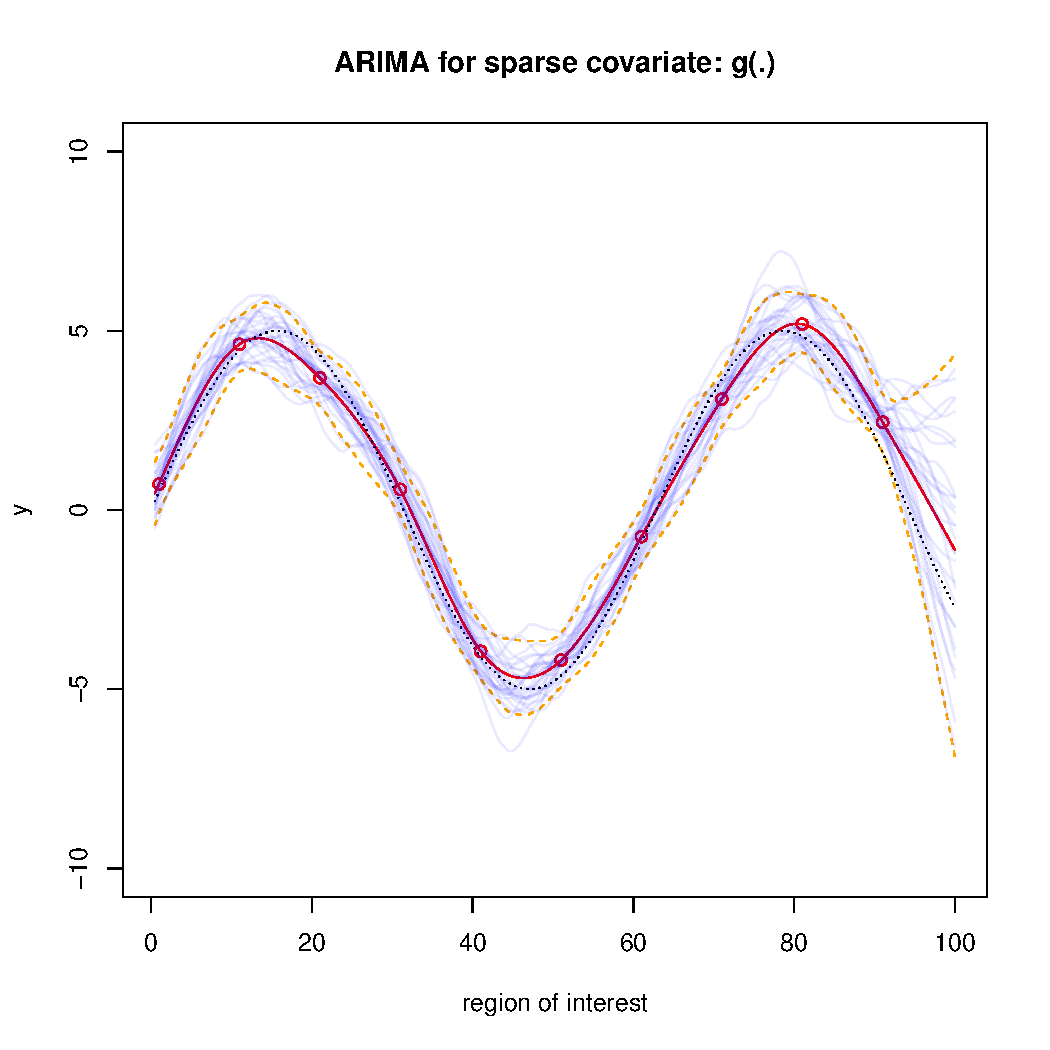
\includegraphics[width=0.27\textwidth]{sim1-g-ARIMA.pdf}
    }
         \subfigure[$g'$ inferred using ARIMA]{
      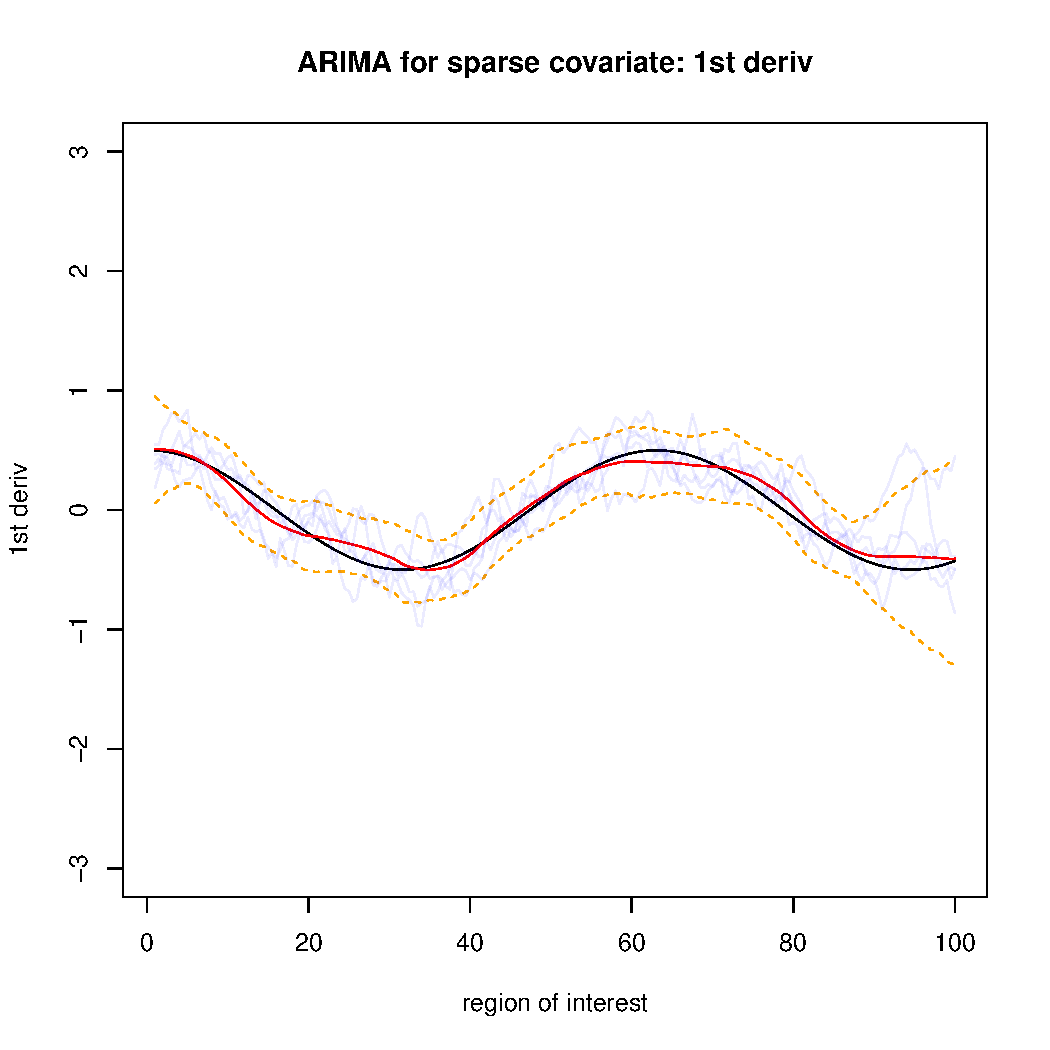
\includegraphics[width=0.27\textwidth]{sim1-g1st-ARIMA.pdf}
    }
     \subfigure[$g''$ inferred using ARIMA]{
      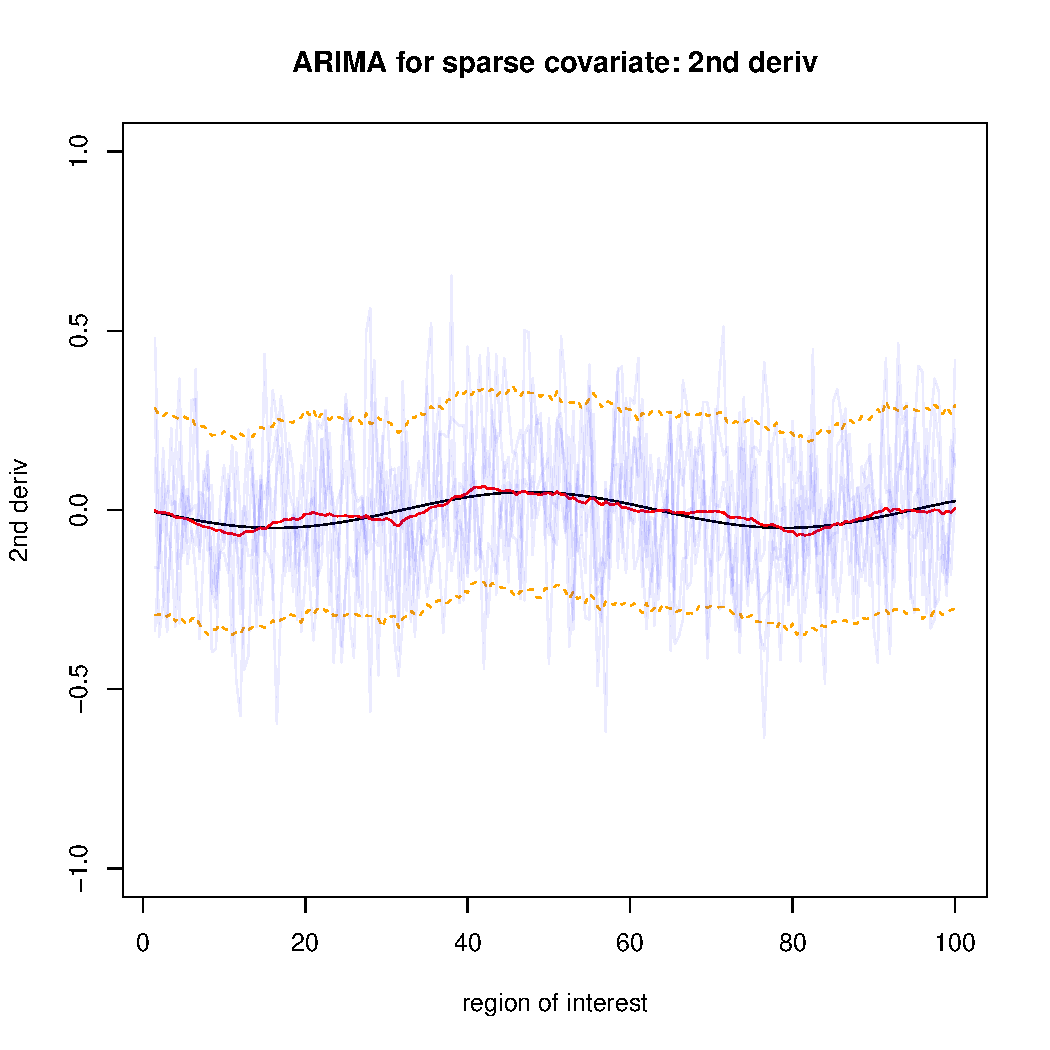
\includegraphics[width=0.27\textwidth]{sim1-g2nd-ARIMA.pdf}
    }
    \label{fig:sim1-1replic}
\end{figure}
\end{frame}


\begin{frame}


\begin{figure}[p]
    \centering
    \subfigure[MCI for $g$]{
      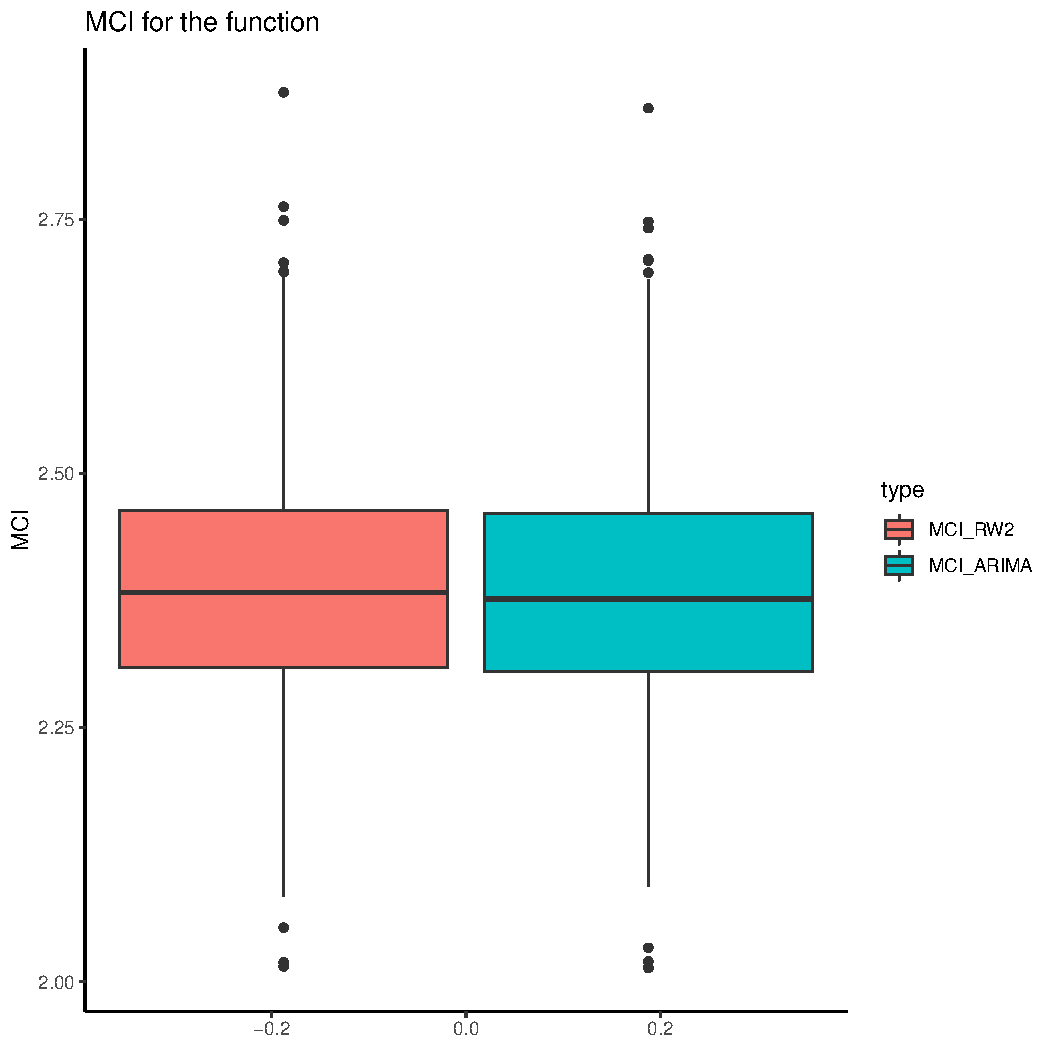
\includegraphics[width=0.29\textwidth]{sim1-g-MCI.pdf}
    }
    \subfigure[MCI for $g'$]{
      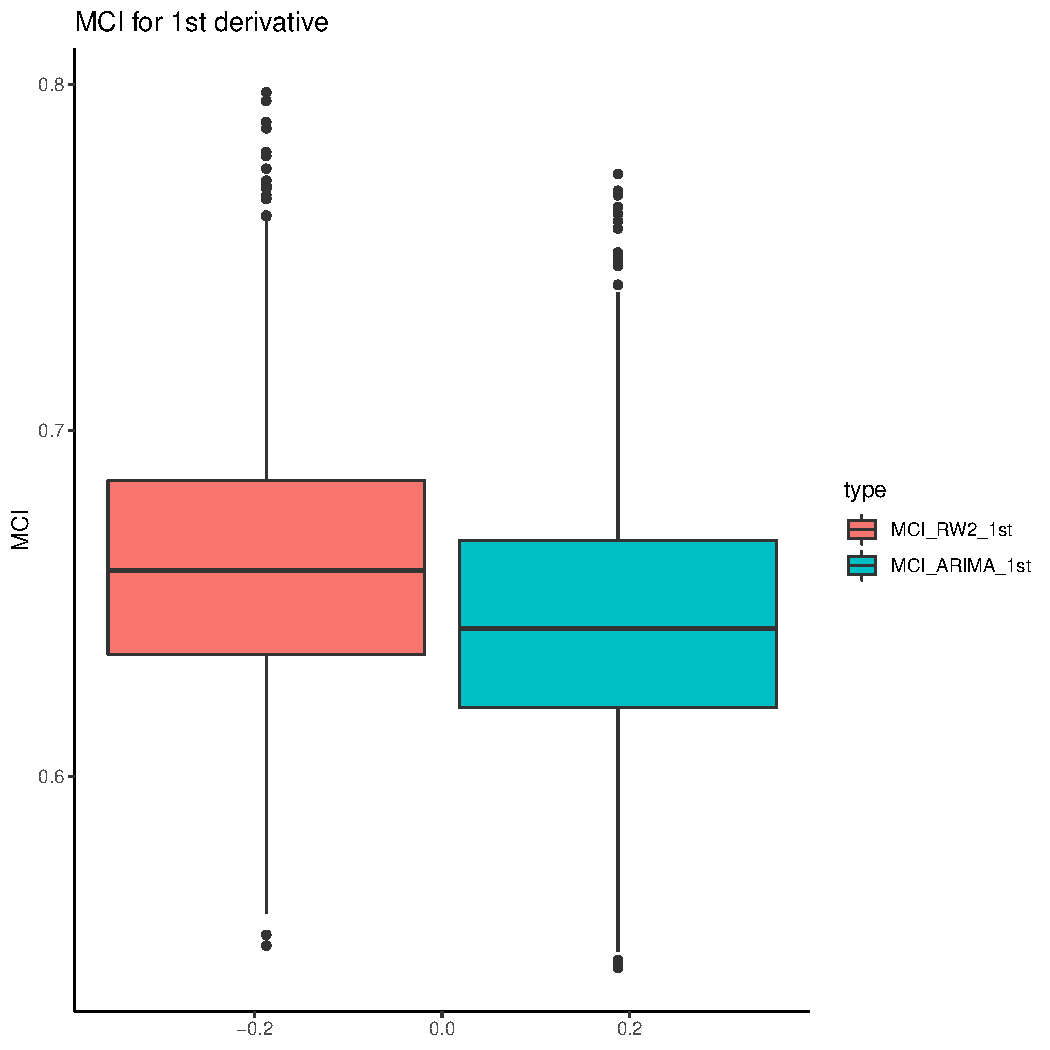
\includegraphics[width=0.29\textwidth]{sim1-g1st-MCI.pdf}
    }
     \subfigure[MCI for $g''$]{
      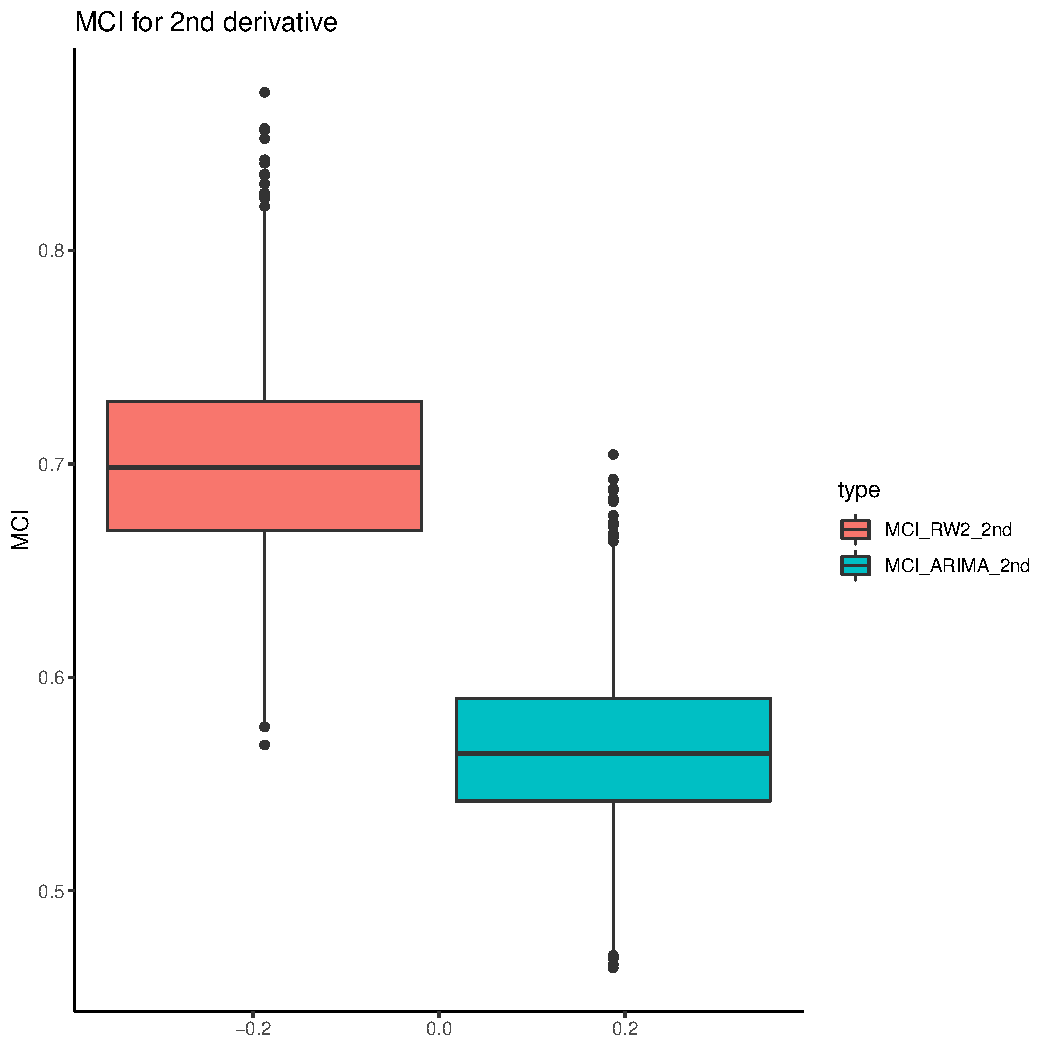
\includegraphics[width=0.29\textwidth]{sim1-g2nd-MCI.pdf}
    }
    \subfigure[CR for $g$]{
      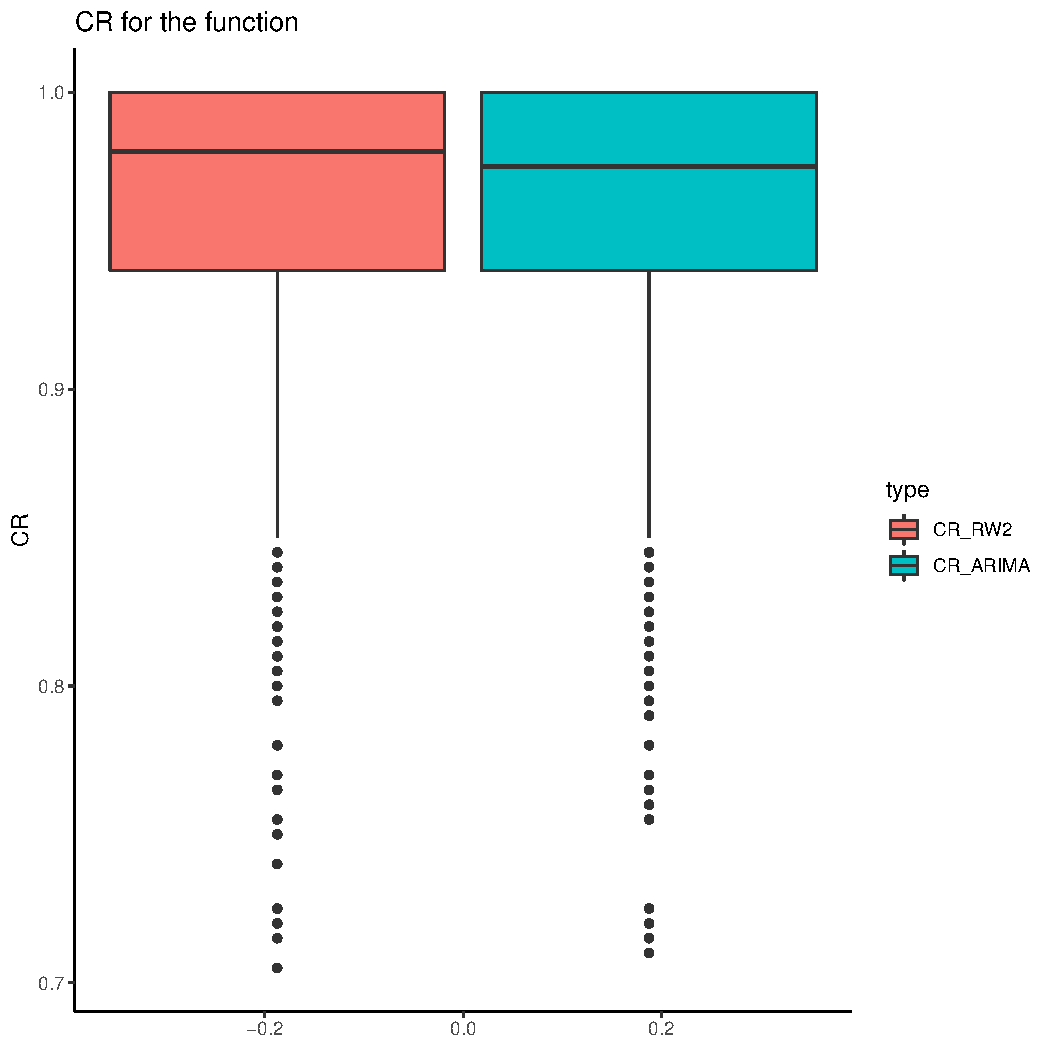
\includegraphics[width=0.29\textwidth]{sim1-g-CR.pdf}
    }
     \subfigure[CR for $g'$]{
      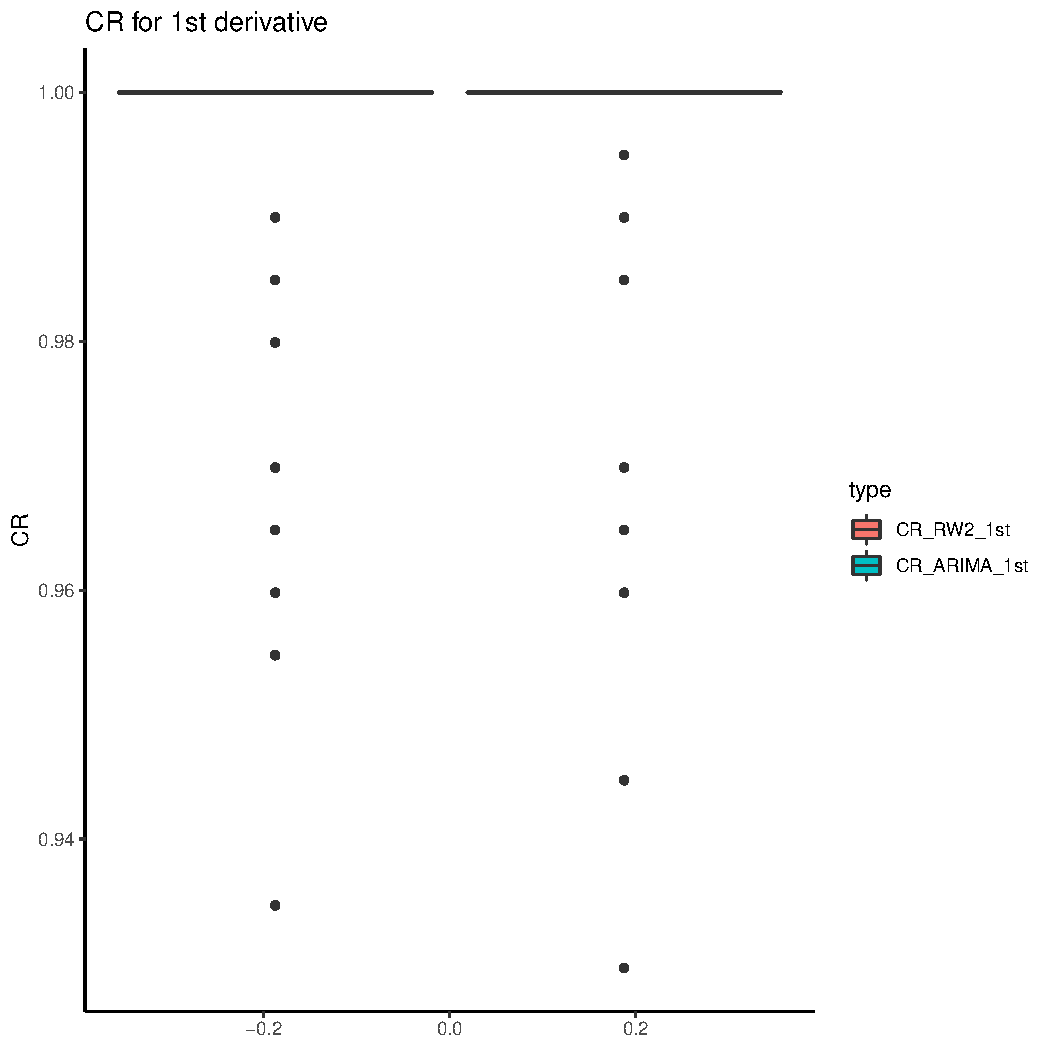
\includegraphics[width=0.29\textwidth]{sim1-g1st-CR.pdf}
    }
     \subfigure[CR for $g''$]{
      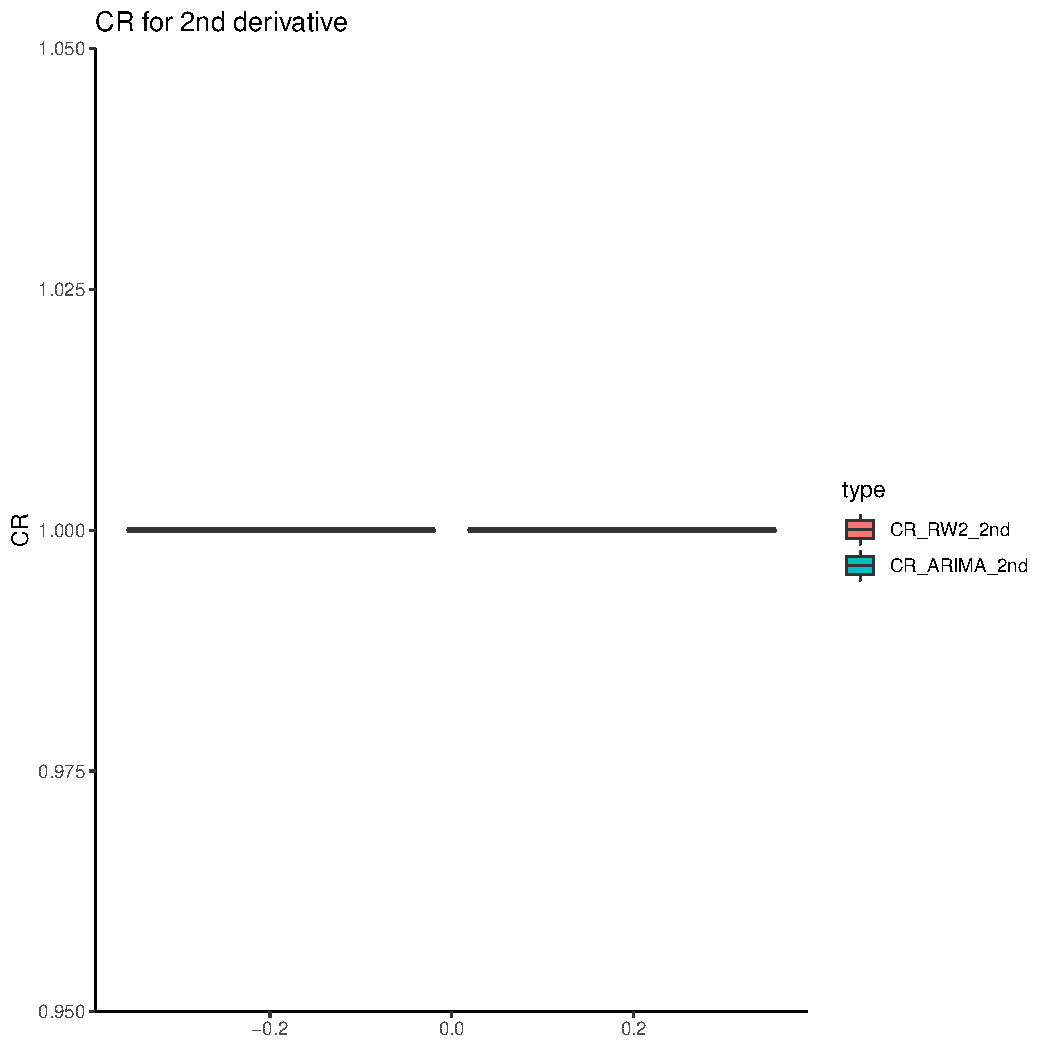
\includegraphics[width=0.29\textwidth]{sim1-g2nd-CR.pdf}
    }
    \caption{Inference for $g,g',g''$ using different methods for the simulation, being replicated for 1000 independent data sets.}
    \label{fig:sim1-1000replic}
\end{figure}


\end{frame}


\subsection{C02 Concentration Data}

\begin{frame}
We illustrate the utility of the two Bayesian smoothing methods described above, using the atmospheric Carbon Dioxide (CO2) concentrations data from an observatory in Hawaii. This dataset contains the observation of CO2 concentrations from 1960 to 2021, with unequally spaced observation times. 
\end{frame}


\begin{frame}
\begin{itemize}

\item We consider the following model: $$y_i = f_{p}(t_i) + f_{np}(t_i) + \epsilon_i,$$ where $y_i$ denotes the observed CO2 concentration at year $t_i$, $f_{p}$ and $f_{np}$ are parametric effects and non-parametric random effects of time $t$.

\pause
\item The parametric effect $f_{p}$ is defined as: $$f_{p}(t) = \beta_0 + \beta_1 \cos(2\pi t) + \beta_2 \sin(2 \pi t) + \beta_3 \cos(4\pi t) + \beta_4 \sin(4\pi t),$$ which aims to capture the deterministic cycles of CO2 variation over time.

\pause
\item The non-parametric effect function $f_{np}(t_i)$ will be inferred using the two Bayesian smoothing methods. For the priors, we use PC prior for the variance parameter $\sigma_\epsilon$ and the smoothing parameter $\sigma_s$, such that $P(\sigma_s > 0.01) = P(\sigma_\epsilon > 1) = 0.5$.

\pause
\item The five fixed effects parameters $\beta_0, ..., \beta_4$ are given independent normal priors with zero mean and variance $10^6$.  

\end{itemize}
\end{frame}





\begin{frame}
We want to consider both the quantity $f_{np}(t)$ and its first/second derivatives for $t \geq 2020$. To better infer the function $f_{np}$, we utilize a resolution grid with equal spacing being 1 week on the time domain, and predict the time domain from the observed years all the way to January 1st of year 2022. 
\end{frame}



\begin{frame}
\begin{figure}[p]
    \centering
         \subfigure[$f'_{np}$ using RW2]{
      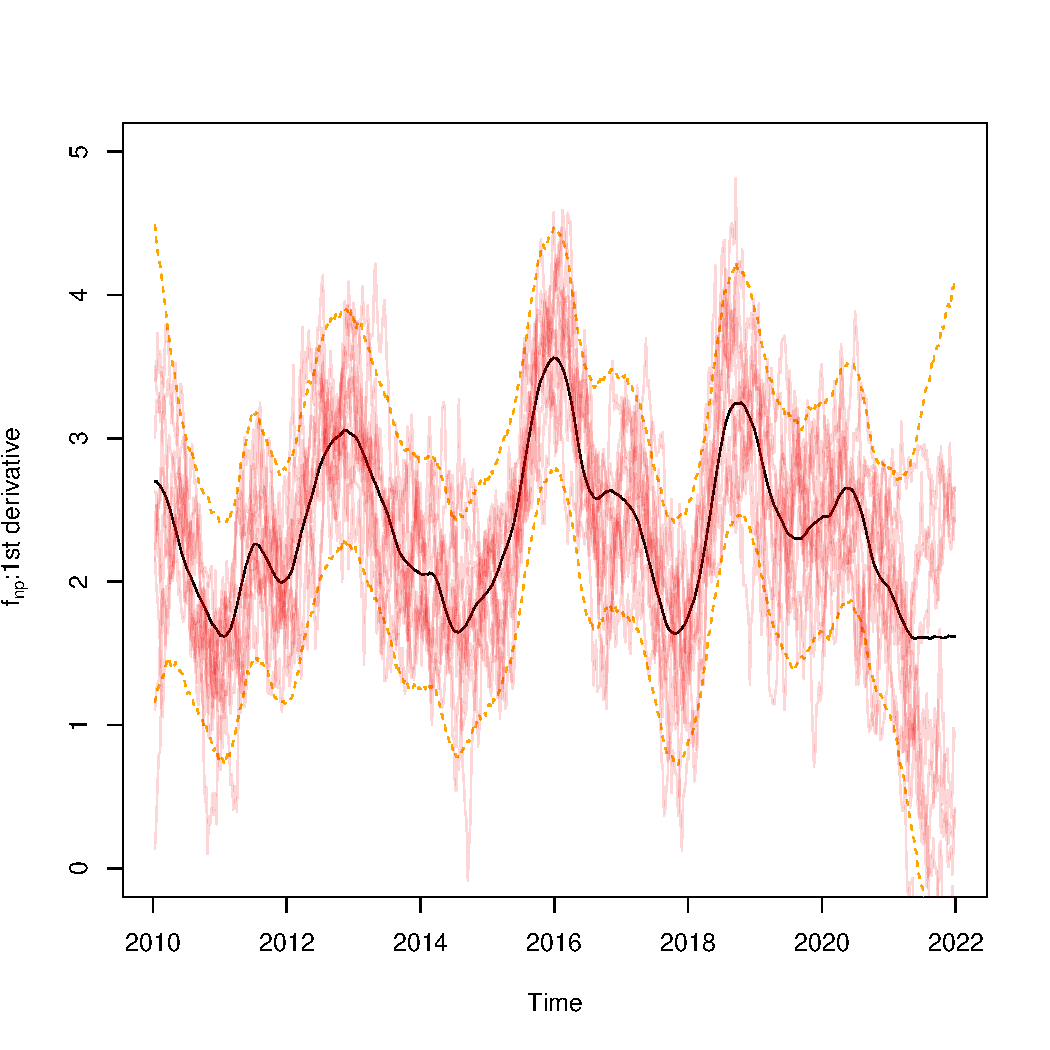
\includegraphics[width=0.3\textwidth]{2010_RW2_1st.pdf}
    }
         \subfigure[$f'_{np}$ using ARIMA]{
      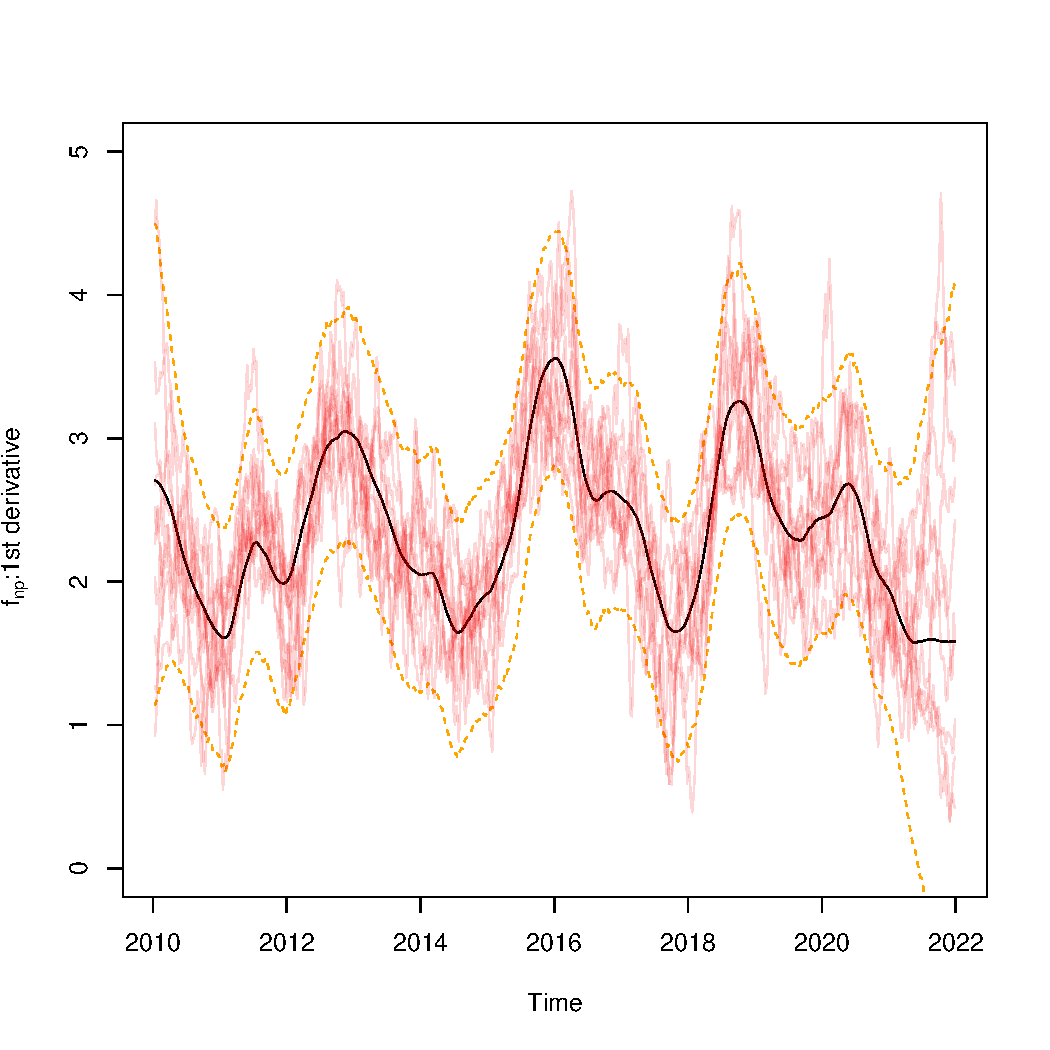
\includegraphics[width=0.3\textwidth]{2010_ARIMA_1st.pdf}
    }
         \subfigure[$f''_{np}$ using RW2]{
      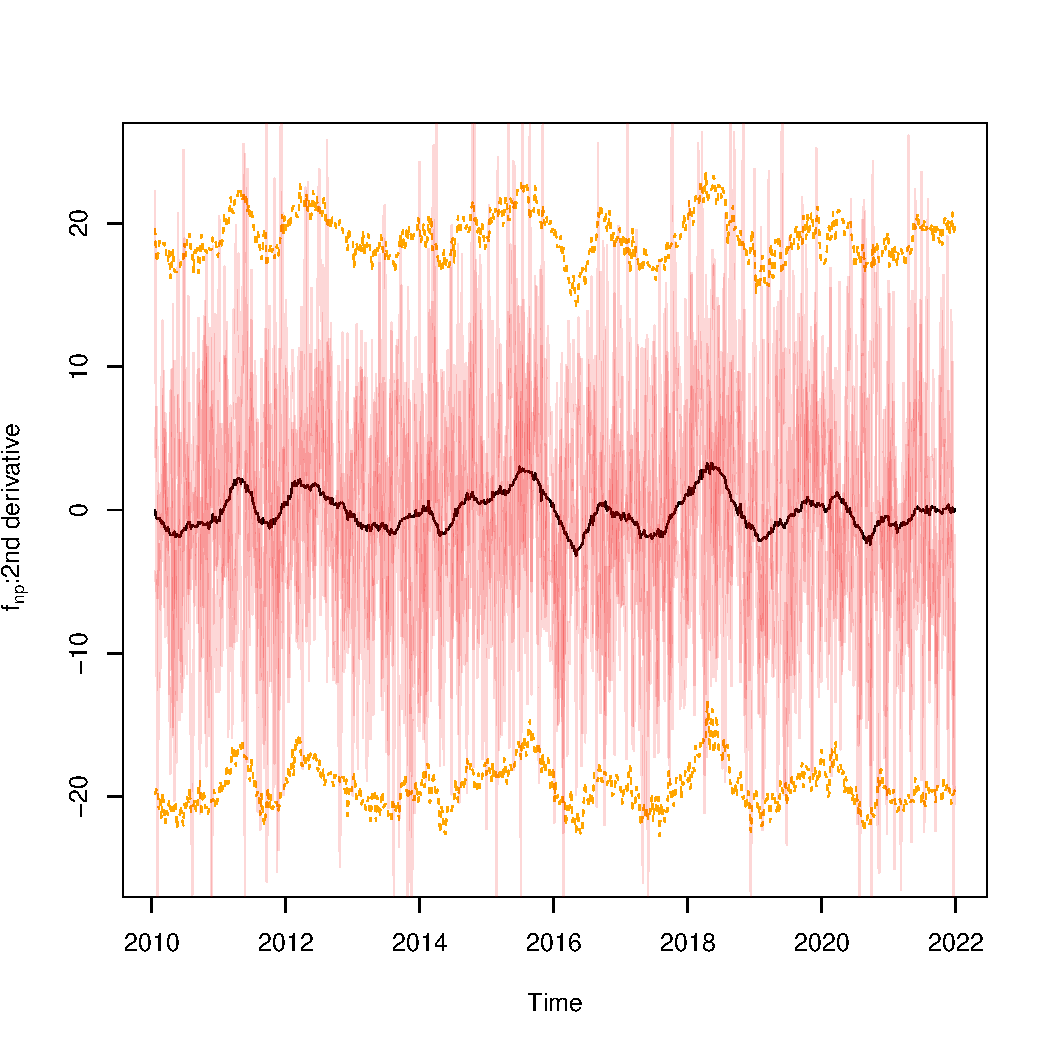
\includegraphics[width=0.3\textwidth]{2010_RW2_2nd.pdf}
    }
             \subfigure[$f''_{np}$ using ARIMA]{
      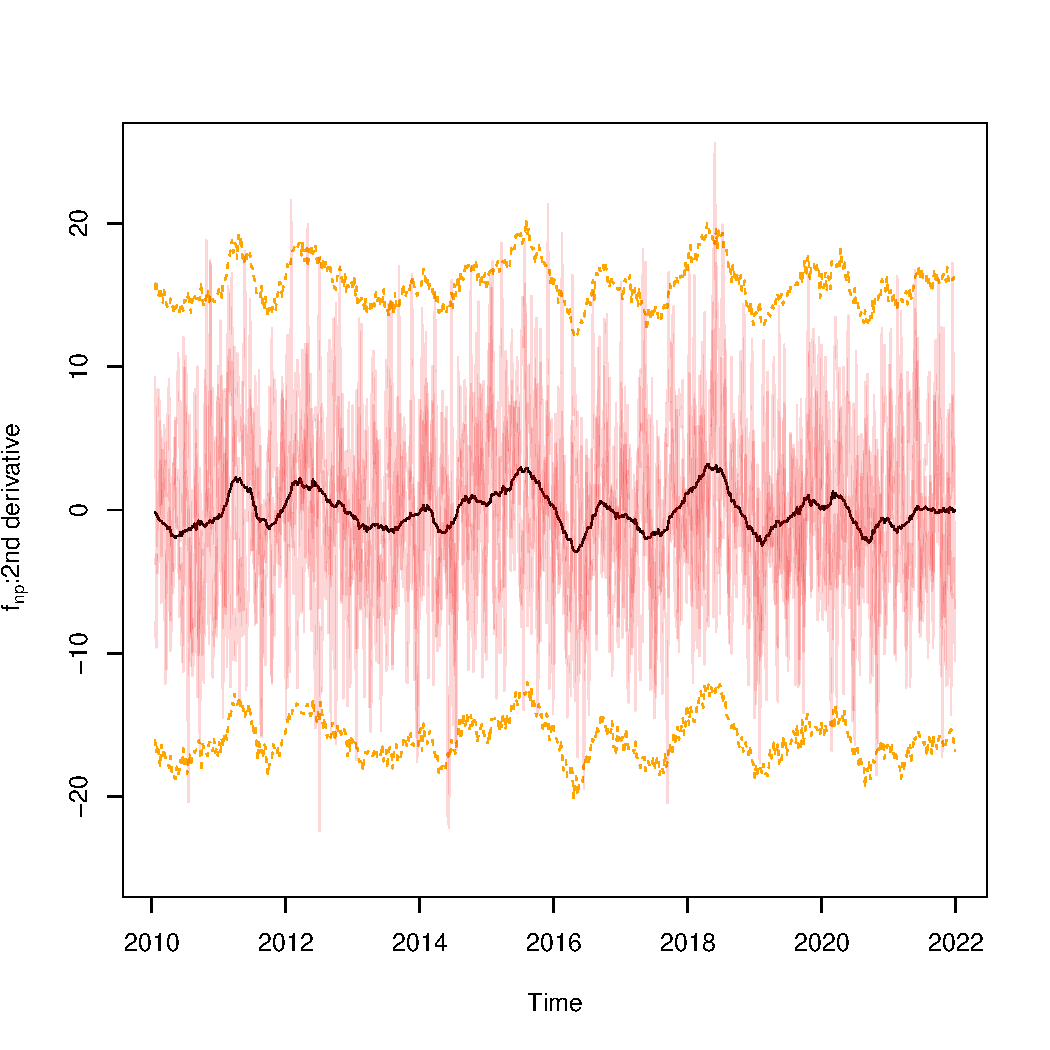
\includegraphics[width=0.3\textwidth]{2010_ARIMA_2nd.pdf}
    }
    \label{fig:realdata_2010}
\end{figure}
\end{frame}





\section{Conclusions}
\begin{frame}
\begin{itemize}

\item We provide an overview of the extended second order random walk method \citep{rw2}, as well as its connection with the smoothing spline \citep{wahba} and the ARIMA prior \citep{ARIMA}.

\pause

\item The extended RW2 method gives similar result in terms of inference for $g$ as the ARIMA method, but at a much smaller computational cost. 

\pause

\item Because of the diagonal approximation it used in the precision matrix, the method gives less smooth inference for higher order derivatives of $g$ compared to ARIMA method.

\pause

\item We illustrate that It is possible to implement the exact ARIMA method without diagonal approximation. But which method is better should depend on the question of interest.

\end{itemize}
\end{frame}



\bibliography{refs}
\bibliographystyle{chicago}


\end{document}